%\input{src/intros/3-soap2p}

\section{P2P networks}
\subsection{P2P definition}
\label{sec:p2p_definition}

A Peer-to-Peer network (onwards called \textit{P2P}) is a distributed system of big scale. His participants
are called \textit{nodes} and they directly share resources and data, acting
like clients and servers. They are called big scale because they are made to
contain millions of nodes through the Internet. Schollmeier at
el~\cite{conf_p2p_Schollmeier01} define P2P networks as:

\numberwithin{mydef}{section}
\begin{mydef}
A distributed network architecture may be called a Peer-to-Peer (P-to-P, PZP,
...) network, if the participants share a part of their own hardware resources (processing power, storage capacity, network link capacity, printers, ...). 
These shared resources are necessary to provide the Service and content offered
by the network (e.g.  file sharing or shared workspaces for collaboration):
They are accessible by other peers directly, without passing intermediary
entities. The participants of such a network are thus resource (Service and
content) providers as well as resource (Service and content) (requestors
(Servent-concept).
\end{mydef}

\subsection{P2P system properties}
\label{sec:p2p_characteristics}

The main properties of a P2P system are:
\begin{enumerate}
    \item \textbf{Scalable}: Can grow \textit{ad infinitum} without compromising its performance.
    \item \textbf{Decentralized}: It does not have a central administration.
    \item \textbf{Heteregeneous}: It is conformed by different devices
connected as \textit{nodes}, with different hardware characteristics each one.
    \item \textbf{Robust}: It is resilient to different types of failures; like
falls and lost of nodes, while maintaining a high data and service availability.
    \item \textbf{Self-organized}: The network structure is maintained and organized by the same nodes that form it, without a manual intervention needed.
\end{enumerate}

\subsection{P2P system structure}
\label{sec:p2p_estructure}

P2P systems are characterized by do not having a central coordination. Each
peer is independent and has a local view of the system. The global behavior
emerges from the local interaction of its members~\cite{Aberer:2001:PIS:503271.503268}.
%El comportamiento global emerge de las interacciones locales
%de sus miembros, y el sistema debe asegurar que toda información y servicio sea
%accesible a pesar de no existir una coordinación central de la
%misma.
Depending in the system topology, they are categorized as structured or
unstructured P2P networks. The structured P2P networks are characterized by a
strong node structure, like a tree or a ring, resulting in additional costs for
each node to maintain the. In unstructured P2P networks the nodes are organized
by simple graphs.

\subsubsection{Unstructured P2P networks}
\label{sec:p2p_unstructured}

\begin{figure}
\center
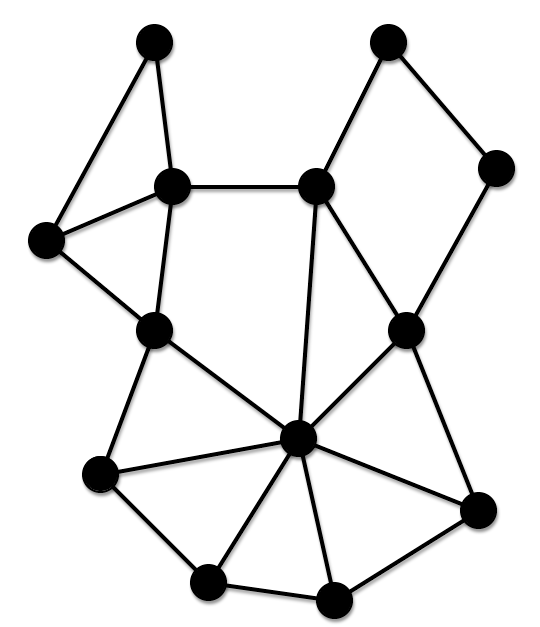
\includegraphics[width=0.5\textwidth]{img/p2p-unstructured}
\caption{Example of unstructured P2P network}
\label{fig:p2p_unstructured}
\end{figure}

%definition
The unstructured systems does not have a strong structure topology. The nodes
establish links in a semi-arbitrary way. Usually, they organize as a hierarchical or a
plain graph.

%advantage
Their main advantage is that they can achieve certain grade of node anonymity.

%disadvantage
The downsize of this type of systems is that searches can end in false
negatives and have a bigger cost in comparison with structured networks. This
is because the search algorithms do not pass through every node inside the
graph.

They are commonly used to share files, using the anonymity of the user to
distribute any type of file through the net.

% examples
There are many implementations of unstructured networks:
Gnutella~\cite{oai:CiteSeerXPSU:10.1.1.61.7302}, 
BitTorrent~\cite{bittorrent}, 
%Freenet~\cite{freenet}, 
%Overnet~\cite{overnet}, 
among others. Each one use different ways to organize the nodes, some using a
node hierarchy to facility the searches in the the network, and others simply
does not count with a search method (BitTorrent).

\paragraph{P2P Unstructured Data Storage}
\label{sec:p2p_unstructured_storage}

This systems storage system does not relate with their network topology, and
does not have a fixed procedure for it. In general, when a node asks for data
and copy it, the network use his copy to distribute it with more nodes in the
system. Each user can decide if he want to share a data or not with the system.
That can make some data of the system go unavailable, and the network by its
own does not have a way to control this.


\paragraph{P2P Unstructured Data Search}
\label{sec:p2p_unstructured_search}

There are many ways to make search inside this type of networks. Some of them
are:

\begin{itemize}
    \item \textbf{Flooding}: 
Each node tries to forward every message to every one of its neighbours except
the source node. To avoid some wasted duplicate deliveries and infinite loops,
each message has a \textit{Time To Live} (TTL) that limits the amount of times
that it can be forwarded. This type of searches has a quadratic cost of network
messages, of order O($N^2$), were N is the number of nodes that can route data
inside the network.
    \item \textbf{K-Random Walk}: Similar to the \textit{flooding} method, with
the difference that each node chooses a number K or a fixed percentage of his
neighbours and forwards the message to the ones that were chosen. When a node
with the required information is found, it responds with a QUERY\_RESPONSE
message following the same way that the Random Walk used to reach him, back to
the original node that started the search. The message cost of this searches
depends of the value of K, approaching:

\numberwithin{equation}{subsection}
\begin{equation}
\label{eq:krandomwalk}
 C = 2 + TTL +
\sum_{i=0}^{TTL} K^i
\end{equation}

\end{itemize}

A way to reduce the message cost in this type o searches, \textit{caching}
techniques can be used, saving the location of the files shared in the network
as they are distributed in it.

\subsubsection{Structured P2P networks}
\label{sec:p2p_estructured}

\begin{figure}
\center
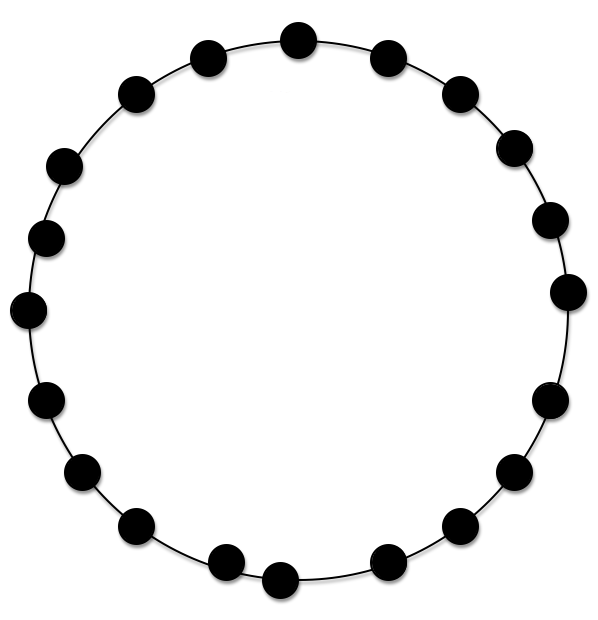
\includegraphics[width=0.5\textwidth]{img/p2p-structured}
\caption{Example of structured network}
\label{fig:p2p_estructured}
\end{figure}


%definition
The structured networks have a strong topology structure. While most of them
use ring structures, other base his topology in binary trees or other
structures to organize.

%advantages
The main advantage of this systems is the search of information. The data search does not
suffer of false negatives, and is more efficient in message cost and response
time than the unstructured ones. 

%disadvantages
As the nodes can be found and traced easily with a query, user anonymity is harder to
achieve in this type of systems.  The applications that want to maintain user
anonymity from his users, this is one of the main reasons to not use this type
of systems.

% examples
The vast majority of structured P2P systems use distributed hash tables
(DHT)~\footnote{http://en.wikipedia.org/wiki/Distributed\_hash\_table} as
structural base for the search and storage system~\cite{BalakrishnanEtAl03}.
CHORD~\cite{conf:hotos:DabekBKKMSB01},
PASTRY~\cite{oai:CiteSeerPSU:441779} and 
OpenDHT~\cite{Rhea:2005:OPD:1080091.1080102}
are some of the systems that are DHT based.

The following work will be based in structured P2P networks, because unstructured
systems does not have the desired properties for the implementation of a
identification system. 

\paragraph{Chord}
\label{sec:chord}

Is a protocol for the implementation of DHT networks that relates a key with
each node. It is design to work in decentralized networks without the use of
special nodes (like super-nodes to help the realization of queries). His
architecture is made to have a basic operational cost proportional to $log(N)$,
with $N$ being the number of nodes in the network.

The protocol takes in consideration that nodes can be inactive or away one
moment or another. Uses the SHA-1 function to assign identifiers to each node
and keys in the system. The Chord protocol dynamically allocates identifiers to nodes that
join or leaves the network. The rest of tasks and services that the system
would need - like user identification, storage, interfaces, etc.- are
responsibility of other implementations of a higher abstraction level than the
Chord protocol itself.

\label{sec:chord}
\begin{figure}
\center
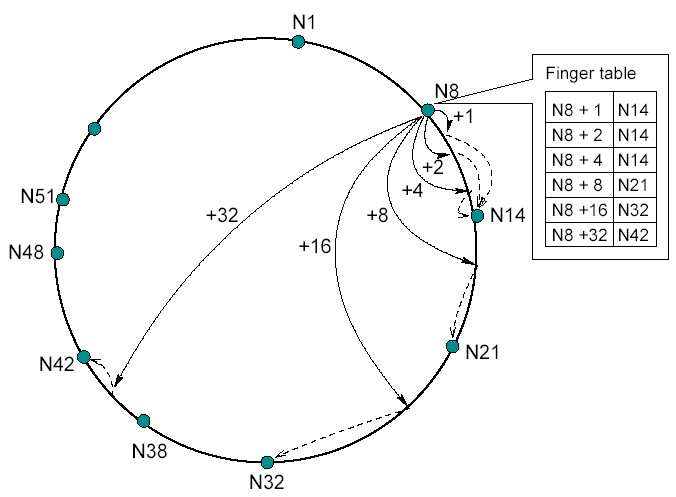
\includegraphics[width=0.5\textwidth]{img/chord-search}
\caption{Chord Routing}
\label{fig:p2p_estructured_chord_search}
\end{figure}

\paragraph{Chord Data Storage}
The network data is stored in the closest node successor of the hash key of the
data. The network search's are made querying the closest successor
nodes that the node has in his \textit{finger table}.
The id key $k$ is assigned to the node id $k$ if this one is active in the
network. If $k$ is not available at that moment, it search for the first node
successor to $k$ that is active and the key id is assigned to him. This
substitute node is denominated \textit{successor of $k$}.
The more close a node id is from other, the more far away physically are the
nodes distributed, giving the network a better resilience to errors.

\paragraph{Chord Information Search}
Key-value pairs are generated using a hash function over each participant of
the network.  Each node register a routing table called \textit{Finger Table}.
In the \textit{Finger Table}, each node register his $i$ successor nodes, each
one being the closest successor to $\theta + 2^{i-1)}$. 
In a search, the number of nodes that a query needs to reach is of order
$O(log(N))$.
The problem that Chord has is that it does not maintain a correlation
between the logical locality of the nodes and their geographical positioning. This
produces that the network communication occurs between nodes very close
logically, but very far physically in the network. While some
optimization's using different heuristics exists to make it better, the locality
problem is not completely fixed.

\paragraph{Pastry}
\label{sec:pastry}
Pastry is a protocol for the DHT implementation. It defines how the node keys id
are distributed and how to find the node responsible of the storage of a key.

\paragraph{Pastry Data Storage}

The data storage is made applying the same hash function used to assign node
identifiers (\textit{nodeID}) to the data filename. This results a key, which is
mapped to a single node. In Pastry, the file is stored in the node that has the closest nodeID
to the data's key.

Exists many replication techniques that manage and distribute copies of the file
in the network. The distribution of the copies is made using the closest nodes
to the chosen node. Using this, if the node in charge of the storage of the file
is missing, the file can still be recovered from his replicas. Also, thanks
to the hash algorithm used, the replicas that are nearby inside the network are
in reality distributed far geographically, improving the data availability
in the system.

\paragraph{Pastry Data Search}

In Pastry, to have an efficient search, each node maintains three data sets:
a routing table, a leafset and a neighbor set.
The leafset is a the set with the closet nodes to the local node, in both
directions of the circle. It serves to maintain the network consistency and
shorten the searches.

The neighbors set are the $m$ closest nodes by the metrics used in the network.
While they are not used by the search algorithm, they helps to maintain the
routing table.
%La búsqueda de información depende del protocolo de red utilizado.
The routing table has a row for each assigned address block. The blocks are
form dividing the nodeID of the local node in digits of $b$ bits. This
generates a numeric system in base $2^b$. In that way, starting at the client,
the nodes are grouped by their number of digits in common in a prefix of the
local node's nodeID and the other node. The table stores in each row the
address of the closest know node, fulfilling the prefix condition of that row.

The messages can be sent to any address in the key space, regardless of whether
the node exists or not. The content is sent through the network until it reaches the node with the given ID (or the closest one, if the exact one does not exist). When a node receives or sends a message, it checks the leafset searching for a direct route. If it does not find one, it sends the message to the known node in the routing table that has  more prexifes in common with the objective. This makes sure that the message will shorten the distance at each step in the search, reaching always the node with the closest nodeID to the objective.

In~\ref{fig:p2p_pastry_routing} we can see an example of the routing algorithm used in Pastry when sending a message.

\begin{figure}
\center
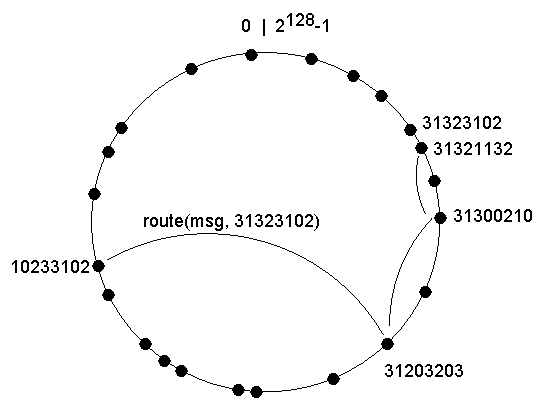
\includegraphics[width=0.6\textwidth]{img/pastryrouting}
\caption{Pastry message routing}
\label{fig:p2p_pastry_routing}
\end{figure}


The search is based in the \textit{lookup(key)}~\cite{BalakrishnanEtAl03} function.
This function takes a \textit{key} and searchs inside of the network a node with
the closest nodeID to the key. If the data exists in the network, the lookup
function returns the node that has it. An important feature of searches in DHT
like Pastry, is that the cost in number of messages is of order $O(log(N))$,
where $N$ is the total number of nodes in the system. Also, it is
\textit{decidable}, meaning that if the data exists in the network, this data
can be found if requested. Other characteristic of the system is his natural
load balancing. The routing algorithm ensures that the request will pass through
a leafset node before reaching the root node, making available for the leafset
node to respond to the request, balancing the load of the request in its
leafset nodes.


%
%
%\paragraph{CAN}
%\label{sec:can}
%%The “Content Addressable Networks” (CAN) [22] work is being done at AT&T Center for Internet Research
%%at ICSI (ACIRI). In the CAN model, nodes are mapped onto a Æ -dimensional coordinate space on top of
%%TCP/IP in a way analogous to the assignment of IDs in Tapestry. The space is divided up into Æ dimensional
%%blocks based on servers density and load information, where each block keeps information on its immediate
%%neighbors. Because addresses are points inside the coordinate space, each node simply routes to the neighbor
%%which makes the most progress towards the destination coordinate. Object location works by the object
%%server pushing copies of location information back in the direction of the most incoming queries.
%%There are several key differences between CAN and Tapestry. In comparison, Tapestry’s hierarchical overlay
%%structure and high fanout at each node results in paths from different sources to a single destination con-
%%verging quickly. Consequently, compared to CAN, queries for local objects converge much faster to cached
%%location information. Furthermore, Tapestry’s use of inherent locality paired with introspective mechanisms
%%means it allows queries to immediately benefit from query locality, while being adaptive to query patterns
%%and allowing consistency issues to be handled at the application layer. CAN assumes objects are immutable,
%%and must be reinserted once they change their values. Finally, Tapestry node organization uses local net-
%%work latency as a distance metric, and has been shown to be a reasonable approximation of the underlying
%%network. CAN, however, like Chord, does not attempt to approximate real network distances in their topol-
%%ogy construction. As a result, logical distances in CAN routing can be arbitrarily expensive, and a hop
%%between neighbors can involve long trips in the underlying IP network. The main advantage a CAN has is
%%that because of the simplicity of the node addition algorithm, it can better adapt to dynamically changing
%%environments such as sensor networks.
%%In summary, Pastry, Chord and CAN are very similar to Tapestry in their functionality and run-time proper-
%%ties. In particular, Pastry is the closest analogy offering “locating and routing” to an object, where Chord and
%%CAN both focus on providing distributed hashtable functionality. Because Pastry controls replica placement,
%%and Chord and CAN are not optimized for large objects, Tapestry is the only system which allows the user
%%to control the location and consistency of the original data, allowing the system to manipulate and control
%%only references to the object for performance. It is also noteworthy that Tapestry and Pastry have natural
%%correlation between the overlay topology and the underlying network distance, while CAN and Chord may
%%incur high physical hop counts for every logical hop.
%
%\begin{figure}
%\center
%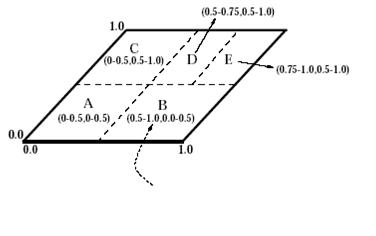
\includegraphics[width=0.6\textwidth]{img/can_structure}
%\caption{Ejemplo de la estructura de CAN}
%\label{fig:can_structure}
%\end{figure}
%
%\paragraph{Almacenamiento de datos}
%En CAN (\textit{Content Addressable Networks}) el espacio de nombres es
%dividido en bloques dimensionales~\ref{fig:can_structure} basándose en la densidad y carga de
%información de los nodos. CAN asume que los objetos son inmutables, y deben ser reinsertados
%una vez que han cambiado sus valores.
%
%\paragraph{Búsqueda de la información}
%Cada bloque mantiene información sobre sus vecinos
%inmediatos. Debido a que las direcciones son puntos dentro del espacio de
%coordenadas, cada nodo simplemente enruta hacia el vecino que realiza el mayor
%progreso frente al del vecino. Una vez que el objeto es encontrado, la
%información es enviada de forma inversa hacia la dirección de más consultas
%realizadas. Al igual que Chord, no mantiene
%correlación entre el espacio de nombres utilizado y la distancia física de los
%nodos, pero su simplicidad le permite adaptarse mejor a ambientes de alto
%dinamismo.
%
%%\paragraph{Skip Graphs}
%%\paragraph{Almacenamiento de datos}
%%\paragraph{Búsqueda de la información}
%
%\paragraph{Tapestry}
%\label{sec:tapestry}
%
%%PAST [11] is a recent project begun at Microsoft Research focusing on peer-to-peer anonymous storage.
%%The PAST routing and location layer, called Pastry [10], is a location protocol sharing many similarities
%%with Tapestry. Key similarities include the use of prefix/suffix address routing, and similar insertion/deletion
%%algorithms, and similar storage overhead costs.
%%There are several key differences that distinquish Pastry from Tapestry. First, objects in PAST are replicated
%%without control by the owner. Upon “publication” of the object, it is replicated and replicas are placed on
%%several nodes whose nodeIDs are closest in the namespace to that of the object’s objectID. Second, where
%
%%Tapestry places references to the object location on hops between the server and the root, Pastry assumes
%%that clients use the objectID to attempt to route directly to the vicinity where replicas of the object are kept.
%%While placing actual replicas at different nodes in the network may reduce location latency, it comes at the
%%price of storage overhead at multiple servers, and brings with it a set of questions on security, confiden-
%%tiality, and consistency. Finally, Pastry routing’s analogy of Tapestry’s “surrogate routing” algorithm (see
%%Section 3.3) provides weaker analytic bounds on the number of logical hops taken. In Tapestry, we have
%%analytically proven, well-defined, probabilistic bounds in routing distances, and are guaranteed to find an
%%existing reachable object (see Section 3).
%
%\paragraph{Almacenamiento de datos}
%Comparte muchas similitudes con Pastry, como su ruteo basado en el
%prefijo de las direcciones, algoritmos similares para la  inserción y borrado y
%costos de almacenamiento de la información.
%Tapestry usa claves numéricas de 160 bits, generadas mediante SHA-1, como
%identificadores tanto de nodos como de objetos dentro de la red. Éstos
%identificadores suelen representarse en formato hexadecimal, siendo más
%próximos dentro del espacio de identificadores contra más dígitos tengan en
%común. 
%Los objetos son publicados enviando un mensaje de publicación hacia el nodo
%raíz correspondiente al hash del objeto. Cada nodo del camino guarda un puntero
%hacia el objeto. Los links redundantes son priorizados por latencia y/o
%localidad.
%
%%De ésta forma, objetos son encontrados realizando consultas hacia la
%%raíz del objeto, en donde cada nodo por el camino revisa sus punteros y
%%redirige la petitición apropiadamente.
%
%%Participants in the network can publish objects by periodically routing a
%%publish message toward the root node. Each node along the path stores a pointer
%%mapping the object. Multiple servers can publish pointers to the same object.
%%The redundant links are prioritized by latency and/or locality. Objects are
%%located by routing a message towards the root of the object. Each node along
%%the path checks the mapping and redirects the request appropriately. The effect
%%of routing is convergence of nearby paths heading to the same destination.
%
%
%\paragraph{Búsqueda de la información}
%
%Un mensaje busca primero un nodo cercano que tenga en común con la clave
%del destino el mismo número en el dígito de menos peso, incrementando
%paulatinamente la parte común hasta encontrar el nodo existente más cercano,
%como se puede visualizar en la figura~\ref{fig:bayeux_routing}.
%
%Para dirigir los mensajes a su destino, Tapestry usa tablas de enrutamiento
%locales en cada nodo, conocidas como \textit{neighbor maps}. La tabla contiene
%múltiples niveles, en donde cada nivel representa un sufijo coincidente hasta
%un dígito. Un nivel dado contiene varias claves, las cuales varían solo en el
%número en la posición indicada por la tabla, similar a la tabla de ruteo
%utilizada por Pastry.
%
%Una búsqueda realiza $O(log_B N)$ saltos en una red de tamaño $N$ y espacio de
%nombres de base $B$. Para un mejor nivel de tolerancia de fallos, se mantiene
%una lista de $c$ links secundarios, de tal forma que la tabla de ruteo posee
%un tamaño de $c B log_B( N)$.

%\red{OTRAS REDES}


